\capitulo{3}{Conceptos teóricos}

\section{Anatomía del iris}
El iris se corresponde con la parte coloreada del ojo, se trata de un músculo circular(o elíptico) protegido por la córnea en cuyo centro se encuentra la pupila. Consta de 2 músculos el \emph{dilatador} y el \emph{esfínter} cuya función es ajustar el tamaño del iris para controlar la cantidad de luz que entra en la pupila.
El conjunto iris-pupila se encuentra rodeado por una membrana de color blanco llamada \emph{esclera}. Ver Figura \ref{fig:eye-anatomy}

El color, la textura y los patrones del iris son únicos y se cree que se forman aleatoriamente durante el periodo embrionario(etapa comprendida entre fecundación y la octava semana de embarazo), de modo que incluso 2 gemelos genéticamente iguales tienen distintos patrones.

En un entorno con mucha luz el esfínter contrae la pupila, dejando pasar menos luz a la retina, mientras que en un entorno poco iluminado, el músculo dilatador, dilata la pupila para permitir la entrada de más luz.
El ojo está protegido externamente por los párpados y las pestañas, sin embargo suponen un problema ya que pueden ocultar significativamente el iris y por tanto resultar en un mal reconocimiento.
%\begin{figure}[h]
%  \centering
%    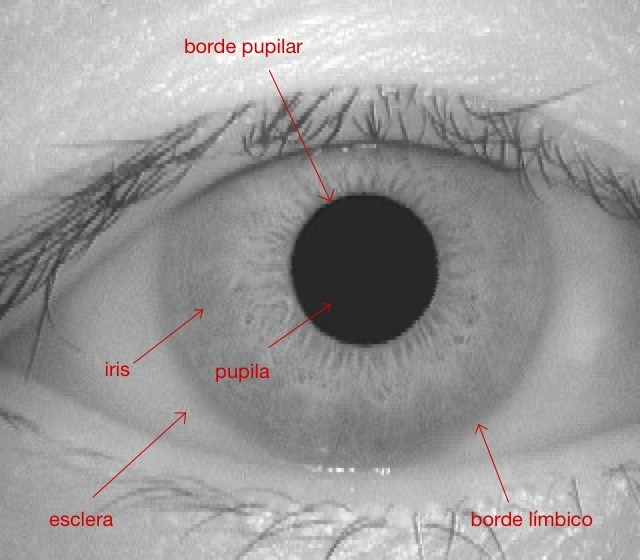
\includegraphics[width=0.7\textwidth]{eye-anatomy}
%  \caption{Imagen 001\_1\_1.bmp del dataset CASIA-Iris V1 que muestra las partes del ojo.}
%\end{figure}
%\newpage
\imagen{eye-anatomy}{Imagen 001\_1\_1.bmp del dataset CASIA-Iris V1 que muestra las partes del ojo.}
\section{Fases del reconocimiento}
Un sistema de reconocimiento tiene 3 fases:
\begin{enumerate}
	\item Adquisición de imágenes.
	\item Preprocesamiento de las imágenes:
	
	La cual se divide en 3 subfases:
	\begin{enumerate}
		\item Segmentación.
		\item Normalización.
		\item Extracción de \emph{features}(patrones del iris)
	\end{enumerate}
	\item Clasificación de las imágenes.

\end{enumerate}

\section{Adquisición de imágenes}
Es la primera de todas las fases y también la más trascendental ya que es necesario que las muestras tengan la calidad necesaria para que la posterior extracción de patrones sea eficiente.

Las muestras de un iris se toman con cámaras desarrolladas específicamente para este propósito si bien para este proyecto no se contaba con este hardware se podría haber optado por usar una cámara convencional(\emph{añadir referencia diabetes bachillerato}), pero ello incluiría otro problema: conseguir muestras de un gran número de voluntarios.
Para evitarse los problemas mencionados se optó por usar un dataset de iris, concretamente el de CASIA en su versión 1(\emph{añadir link a CASIA}) la cual está disponible de forma gratuita mediante registro y autorización previa.

Este dataset cuenta con 756 imágenes del iris de 108 sujetos. La toma de muestras se realizó en 2 sesiones, tomándose 3 muestras en la primera sesión y 4 en la segunda, de modo que se cuenta con un total de 7 muestras por sujeto.
Cada muestra está en formato \emph{.bmp} y tienen una resolución de 320x280.
Para la toma de muestras usaron una cámara desarrollada por la propia CASIA.
\imagen{casia-camera}{Toma de muestras para el dataset CASIA-Iris-V1}
Con el objetivo de facilitar la detección de los bordes del iris, las muestras se han editado, de modo que se han eliminado los reflejos especulares(\emph{añadir pie de página con definición}).

Cabe recalcar que dichas ediciones son mínimas y se aplican únicamente en la pupila, la cual no proporciona ninguna información útil para las etapas posteriores de extracción y clasificación de los patrones del iris.(\emph{añadir referferencia a image understanding for irsi.... }
\imagen{specular}{Imagen S1143R01.jpg perteneciente CASIA-Interval-V3 con regiones especulares(izquierda). Imagen 001\_1\_1.bmp de CASIA-Iris-V1 sin regiones especulares(derecha)}

\section{Preprocesamiento}
Como puede apreciarse en la figura de la derecha de la imagen \ref{fig:specular}, la muestra es del ojo completo, pero para el reconocimiento únicamnete nos interesa la regíón del iris, por lo que elementos como pestañas, párpados, esclera \emph{etc} han de eliminarse ya que no aportan nada.
Así mismo dependiendo de las condiciones en las que se tomaron las muestras es posible que el tamaño de los iris varíe debido a la dilatación o la contracción de la pupila.

Es por ellos que ha de procesarse la imagen para localizar y aislar el iris(\emph{segmentar}) y ajustarlo a un tamaño estándar(\emph{normalizar})


\subsection{Segmentación}
En esta etapa se requiere detectar de manera automática los bordes \emph{límbico} y \emph{pupilar} del ojo aislando la región del iris y excluyendo el resto de la imagen, es decir, se busca el \emph{ROI(Region of interest)}

El iris se corresponde con la región circular comprendido entre la pupila y la esclera.a
La mayoría de fallos en un sistema de reconocimiento de iris se debe a una segmentación deficiente de las imágenes, por lo que se han de tener en cuenta los siguientes factores:
\begin{itemize}
    \item El iris se encuetra obstruido por pestañas, párpados y reflejos especulares.
    \item Tanto iris como pupila no son siempre circulares sino que pueden tener forma elíptica, y su forma puede variar dependiendo de la forma en que se tome la muestra.
    \item Factores cómo muestras desenfocadas, con mucho ruido, poca calidad.. (estos han de tenerse en cuenta en la etapa de adquisición de imágenes)
\end{itemize}

\imagen{segmentado}{Detección incorrecta de los bordes límbico y pupilar (izquierda) y la correcta(derecha)}
Como se ha dicho anteriormente, los algoritmos de Daugman son la base de los sistemas de reconocimiento actuales, pero no son los únicos métodos existentes.

\begin{itemize}
    \item\textbf{Operador Integro-Diferencial de Daugman:} Daugman propuso el primer modelo funcional para un sistema de reconocimiento de iris y consiste en un detector de bordes circulares que busca el máximo valor del cambio de tonalidad en la imagen utilizando la integral de línea de varios círculos concéntricos.
    
    El operador viene determinado por la siguiente ecuación:
    
    \emph{añdir refrencia iris detection and noramlization[4]}
    \begin{equation*}
    \max_{\substack(r,x_{0},y_{0})}\left | G_{\sigma }(r)*\frac{\partial }{\partial x}\oint_{(r,x_{0},y_{0})} \frac{I(x,y)}{2\pi r}ds \right |
    \end{equation*}
    donde $I(x,y)$ se corresponde con la imagen del ojo, $ds$ es el arco diferencial del círculo de radio $r$ y coordenadas $(x_{0},y_{0})$. $G_{\sigma}$
    es una función que suaviza la imagen como un filtro Gaussiano de tamaño $\sigma$. Dado que utiliza información derivativa de primer orden, se computa muy rápidamente.\emph{refrencia a http://repositorio.uchile.cl/handle/2250/132304}
    \textbf{NOTA JOHNSON: no voy a usar ese método, sin embargo lo he puesto solo de relleno cosa que no sé si está bien o mal, además soy incapaz de comprender la ecuación en sí misma, así que he copiado literalmente lo que aparecía en el artículo citado}
    \item\textbf{Transformada de Hough:} parte de la idea de que los bordes límbico y pupilar pueden ser considerados como círculos, la Transformada de Hough original se usaba en un principio para la detección de líneas en una imagen, sin embargo más adelante se extendió para que pudiera reconocer también circulos y circunferencias, pasó a denominarse \emph{Transformada de Hough Circular}.
    Su funcionamietno es el siguiente:
    Primero se genera el \emph{edge map} de la imagen mediante el cáclculo de la primera derivada de las intensidades de los valores y a continuación se establece un umbral umbral\emph{thresholding}. Posteriormente se suaviza la muestra con un filtro Gaussiano.
    
    \textbf{NOTA JOHNSON: sé lo que hace, pero no sé cómo traducirlo ya que es muy técnico, referencia-> Iris detection and normalization}
    
    \item\textbf{Detectector de bordes de Canny:} se basa en detección de contornos mediante el uso de máscaras de convolución y el cálculo de la primera derivada.
    Los puntos que conforman los bordes detectados se consideran zonas de píxeles en los que existe un cambio brusco del nivel de gris\emph{referencia a Detección de bordes mediante el algoritmo de Canny}
\end{itemize}

El método seguido para la realización de este proyecto se basa en el propuesto por Wildes \emph{referencia Iris recognition: an emerging biometric technology.} 

Wildes propone utilizar el detector de bordes de Canny seguido de la Transformada de Hough Circular, la combinación de ambos métodos proporciona resultados que pueden superar a los de Daugman.

Para su correcta aplicación se ha de buscar un valor de \emph{thresholding} común para la pupila y el iris, y posteriormente detectar los bordes, por lo que serán necesarios como mínimo 2 iteraciones, la primera para detectar el borde límbico y la segunda para detectar el borde pupilar.

Wildes sugiere empezar por el borde exterior(el límbico), por lo que primero se calculará el umbral apropiado para binarizar la imagen y una vez calculado se usará para detectar los bordes con Canny.
Se usó el método \emph{.Canny()} de la librería de 
\emph{OpenCV} para facilitar el proceso.

\subsubsection{Detección del borde límbico}
\imagen{thresh-canny-limbic}{Imagen binarizada(\emph{izquierda}). Imagen con bordes detectados con Canny(\emph{derecha})}

\imagen{draw-lines-limbic}{Circunferencia exterior dibujada sobre el \emph{edge map} y sobre la muestra original.}

El proceso de detección del borde límbico se corresponde con la primera iteración, la detección del borde pupilar, se corresponde con la segunda y los pasos a realizar son iguales, ya que  lo único que se necesitará es ajustar los umbrales.

\subsubsection{Detección del borde pupilar}

\imagen{thresh-canny-pupilar}{Imagen binarizada(\emph{izquierda}). Imagen con bordes detectados con Canny(\emph{derecha})}

\imagen{draw-lines-pupilar}{Circunferencia interior dibujada sobre el \emph{edge map} y sobre la muestra original.}


Para ejemplificar el proceso que se ha de seguir para encontrarr los bordes, se ha trabajado sobre la muestra \emph{001\_1\_1.bmp} de CASIA-Iris-V1, aunque a priori parecía que el proceso desarrollado podría aplicarse a todas las muestras del dataset, más tarde se comprobó que no era así ya que existían fallos principlamente para detectar el borde exterior.
\subsection{Detección de bordes errónea}
\imagen{wrong-borders-2}{Imagen \emph{002\_1\_1.bmp}, debido a la mala binarización interpreta la pupila como el iris.}
\imagen{wrong-borders-pupil-2}{Imagen \emph{002\_1\_1.bmp}, pupila detectada correctamente}
\imagen{wrong-borders-8}{Imagen \emph{008\_1\_1.bmp}, debido a la mala binarización dibuja la circunferencia en una región aleatoria.}
\imagen{wrong-borders-pupil-8}{Imagen \emph{008\_1\_1.bmp}, pupila detectada correctamente.}

Por lo tanto se llega a la conclusión que es posible aplicar un \emph{thresholding} común para todas las muestras pero únicamente para la detección de la pupila, mientras que para la detección del iris, se deberá ir probando constantemente hasta encontrar el apropiado para cada imagen, esto se correspondería con una técnica de fuerza bruta muy ineficiente, que podría ser factible si se cuenta con un dataset pequeño, pero para el de CASIA que cuenta con 108 muestras no lo es.

Para paliar este problema se emplea una \emph{red neuronal preentrenada -> enlace https://github.com/jus390/U-net-Iris-segmentation} que permitirá la segmentación automática.




